% documentclass: article used for scientific journals, short reports, program documentation, etc
% options: fontsize 11, generate document for double sided printing, a4-paper
\documentclass[10pt, twoside, a4paper, fleqn]{article}

% package for changing page layout
\usepackage{geometry}
\geometry{a4paper, lmargin=40mm, rmargin=45mm, tmargin=40mm, bmargin=45mm}
% set indentation
\setlength{\parindent}{1em}
% set factor for line spacing
% \linespread{1.0}\selectfont
% set (dynamic) additional line spacing
% \setlength{\parskip}{1ex plus 0.5ex minus 0.3ex}

% rigorous formatting (not too much hyphens)
% \fussy
% \sloppy

% package for changing page layout (used to indent whole paragraphs with adjustwidth)
\usepackage{changepage}

% input encoding for special characters (e.g. ä,ü,ö,ß), only for non english text
% options: utf8 as encoding standard, latin1
\usepackage[utf8]{inputenc}
% package for font encoding
\usepackage[T1]{fontenc}
% package for changing used language (especially for more than one language)
% options: ngerman (new spelling) or default: english
\usepackage[ngerman]{babel}
% package for times font
% \usepackage{times}
% package for latin modern fonts
\usepackage{lmodern}

% package for math symbols, functions and environments from ams(american mathematical society)
\usepackage{amsmath}
\usepackage{mathtools}
% package for extended symbols from ams
\usepackage{amssymb}
% package for math black board symbols (e.g. R,Q,Z,...)
\usepackage{bbm}
% package used for calligraphic math symbols
\usepackage{mathrsfs}
% package for extended symbols from stmaryrd(st mary road)
\usepackage{stmaryrd}
% package for more math blackboard symbols
\usepackage{dsfont}

% pack­age im­ple­ments scal­ing of the math ex­ten­sion font cmex; used for scaling math signs
\usepackage{exscale}

% package for including extern graphics plus scaling and rotating
\usepackage{graphicx}
%package for positioning figures
\usepackage{float}
% package for changing color of font and paper
% options: using names of default colors (e.g red, black)
% \usepackage[usenames]{color}
\usepackage[dvipsnames]{xcolor}
\definecolor{shadecolor}{gray}{0.9}
% package for customising captions
\usepackage[footnotesize, hang]{caption}
% package for customising enumerations (e.g. axioms)
\usepackage{enumitem}
% calc package reimplements \setcounter, \addtocounter, \setlength and \addtolength: commands now accept an infix notation expression
\usepackage{calc}
% package for creating framed, shaded, or differently highlighted regions that can break across pages; environments: framed, oframed, shaded, shaded*, snugshade, snugshade*, leftbar, titled-frame
\usepackage{framed}
% package for creating custom "list of"
% options: titles: do not intefere with standard headings for "list of"
\usepackage[titles]{tocloft}
% change enumeration style of equations
% \renewcommand\theequation{\thesection.\arabic{equation}}

% init list of math for definitions and theorems
\newcommand{\listofmathcall}{Verzeichnis der Definitionen und Sätze}
\newlistof{math}{mathlist}{\listofmathcall}
% add parentheses around argument
\newcommand{\parent}[1]{ \ifx&#1&\else (#1) \fi }
\definecolor{mathdefback}{rgb}{0.95,0.95,0.98}
% unnumerated mathematical definition environment definiton
\newenvironment{mathdef*}[2]{
	\medskip
	\begin{tcolorbox}[colback=mathdefback, boxrule=0.5pt, colframe=black, boxsep=0pt, enhanced jigsaw, breakable, arc=3pt]
	\noindent
	{ \fontfamily{ppl}\selectfont \textbf{\textsc{#1:}} } ~ #2 
	\par \hfill\\ 
	\fontfamily{lmr}\selectfont \itshape
}{
	\end{tcolorbox}
	\medskip
}
% definitions for numerated mathematical definition environment
\newcounter{mathdefc}[section]
\newcommand*{\mathdefnum}{\thesection.\arabic{mathdefc}}
\renewcommand{\themathdefc}{\mathdefnum}
\newenvironment{mathdef}[2]{
	\refstepcounter{mathdefc}
	\addcontentsline{mathlist}{figure}{\protect{\numberline{\mathdefnum}#1 ~ #2}}
	\begin{mathdef*}{#1 \mathdefnum}{#2}
}{
	\end{mathdef*}
}
% standard mathdef calls
\newcommand{\definitioncall}{Definition}
\newenvironment{definition*}[1][]{ \begin{mathdef*}{\definitioncall}{\parent{#1}} }{ \end{mathdef*} }
\newenvironment{definition}[1][]{ \begin{mathdef}{\definitioncall}{\parent{#1}} }{ \end{mathdef} }

\definecolor{maththeoremframe}{rgb}{0.7,0.7,0.73}

% unnumerated theorem environment definition
\newenvironment{maththeorem*}[2]{
	\medskip
	\begin{tcolorbox}[boxrule=0pt, leftrule=2.5pt, arc=2pt, colback=white, colframe=maththeoremframe, enhanced jigsaw, breakable, vfill before first, top=0mm, bottom=0mm, left=2mm, right=0mm, boxsep=1mm]
	\noindent
	{ \fontfamily{ppl}\selectfont \textbf{\textsc{#1:}} } ~ #2
	\par \hfill\\ 
	\fontfamily{lmr} \fontshape{it} \selectfont
}{ 
	\end{tcolorbox}
	\medskip
}
% definitions for numerated theorem environment
\newcounter{maththeoremc}[section]
\newcommand*\maththeoremnum{\thesection.\arabic{maththeoremc}}
\renewcommand{\themaththeoremc}{\maththeoremnum}
\newenvironment{maththeorem}[2]{
	\refstepcounter{maththeoremc}
	\addcontentsline{mathlist}{figure}{\protect{\qquad\numberline{\maththeoremnum}#1 ~ #2}}
	\begin{maththeorem*}{#1 \maththeoremnum}{#2}
}{
	\end{maththeorem*}
}
% standard maththeorem calls
\newcommand{\theoremcall}{Theorem}
\newenvironment{theorem*}[1][]{ \begin{maththeorem*}{\theoremcall}{\parent{#1}} }{ \end{maththeorem*} }
\newenvironment{theorem}[1][]{ \begin{maththeorem}{\theoremcall}{\parent{#1}} }{ \end{maththeorem} }
\newcommand{\lemmacall}{Lemma}
\newenvironment{lemma*}[1][]{ \begin{maththeorem*}{\lemmacall}{\parent{#1}} }{ \end{maththeorem*} }
\newenvironment{lemma}[1][]{ \begin{maththeorem}{\lemmacall}{\parent{#1}} }{ \end{maththeorem} }
\newcommand{\propositioncall}{Proposition}
\newenvironment{proposition*}[1][]{ \begin{maththeorem*}{\propositioncall}{\parent{#1}} }{ \end{maththeorem*} }
\newenvironment{proposition}[1][]{ \begin{maththeorem}{\propositioncall}{\parent{#1}} }{ \end{maththeorem} }
\newcommand{\corollarycall}{Korollar}
\newenvironment{corollary*}[1][]{ \begin{maththeorem*}{\corollarycall}{\parent{#1}} }{ \end{maththeorem*} }
\newenvironment{corollary}[1][]{ \begin{maththeorem}{\corollarycall}{\parent{#1}} }{ \end{maththeorem} }
% q.e.d. definition
\newcommand{\qed}{ \par \hfill \fontfamily{lmr} \fontshape{it} \selectfont \mbox{q.e.d.} \\}
\newcommand{\qedbox}{ \hfill $\Box$ }
% proof environment definition for theorems
\newenvironment{mathproof}[2]{
	% \par\hfill\\
	\medskip
	% \noindent
	% \par
	% { \fontfamily{ppl}\selectfont \small \textsc{#1:} } ~ \parent{#2} \smallskip\\
	% \begin{adjustwidth}{1em}{}
	\begin{tcolorbox}[title= { \fontfamily{ppl}\selectfont \small \textsc{#1:} } ~ \parent{#2}, boxrule=0pt, colback=white, colframe=white, coltitle=black, breakable, boxsep=0mm, top=2mm, bottom=0mm, right=0mm, left=0mm, before upper={\parindent1em}]%
	\normalfont
	\small
}{ 
	\end{tcolorbox}
	% \end{adjustwidth} 
	% \qedbox
	\medskip
}
% standard mathproof calls
\newcommand{\proofcall}{Beweis}
\newenvironment{proof}[1][]{ \begin{mathproof}{\textbf{\proofcall}}{#1} }{ \qedbox \end{mathproof} }
\newcommand{\proofideacall}{Beweisidee}
\newenvironment{proofidea}[1][]{ \begin{mathproof}{\proofideacall}{#1} }{ \end{mathproof} }
\newcommand{\examplecall}{Beispiel}
\newenvironment{example}[1][]{ \begin{mathproof}{\examplecall}{#1} }{ \end{mathproof} }

% new displaymath command, so that equations will not be stretched
\newcommand{\D}[1]{\mbox{$ #1 $}}
% make unnumerated equation
\newcommand{\E}[1]{\[ #1 \]}
% command for curly brackets
\newcommand{\curlb}[1]{\left\{ #1 \right\}}
% command for box brackets
\newcommand{\boxb}[1]{\left[ #1 \right]}
% command for parentheses/curved brackets
\newcommand{\curvb}[1]{\left( #1 \right)}
% command for angle brackets
\newcommand{\angleb}[1]{\left\langle #1 \right\rangle}
% command for floor brackets
\newcommand{\floorb}[1]{\left\lfloor #1 \right\rfloor}
% command for ceil brackets
\newcommand{\ceilb}[1]{\left\lceil #1 \right\rceil}
% command for creating sets
\newcommand{\set}[2]{ \left\{ #1 \enspace \middle\vert \enspace #2 \right\} }
% command for absolute value
\newcommand{\abs}[1]{\left\vert #1 \right\vert}
\newcommand{\norm}[1]{\left\| #1 \right\|}
% commands for writing limits
\newcommand{\limit}[3]{\, \longrightarrow \, #1, \ #2 \longrightarrow #3}
\newcommand{\Limit}[2]{\lim_{#1 \rightarrow #2}}
% command for differential
\newcommand{\diff}{\mathrm{d}}
\newcommand{\Diff}{\mathrm{D}}
% command for derivative
% \newcommand{\Deriv}[3][]{\Diff_{#2}^{#1}#3}
% \newcommand{\deriv}[3][]{\dfrac{\diff^{#1}#2(#3)}{\diff #3^{#1}}}
% command for integral
\newcommand{\integral}[4]{\int_{#1}^{#2} #3\ \diff #4}
\newcommand{\Integral}[4]{\int\limits_{#1}^{#2} #3\ \diff #4}
\newcommand{\iintegral}[2]{\int #1\ \diff #2} % indefinite integral
% mathematical definitions (standard sets)
\newcommand{\SR}{\mathds{R}} % real numbers
\newcommand{\SC}{\mathds{C}} % complex numbers
\newcommand{\SN}{\mathds{N}} % natural numbers
\newcommand{\SZ}{\mathds{Z}} % integral numbers
\newcommand{\SQ}{\mathds{Q}} % rational numbers
\newcommand{\SP}{\mathcal{P}} % power set
\newcommand{\SFP}{\mathds{P}} % polynom functions
\newcommand{\SFC}{\mathrm{C}} % complex valued functions (continous or differentiable)
\newcommand{\SFL}{\mathcal{L}} % space of integrable functions
\newcommand{\SFLL}{\mathrm{L}} % space of integrable function classes
\newcommand{\SH}{\mathcal{H}} % hilbert space
% mathematical standard functions
\DeclareMathOperator{\real}{Re} % real part
\DeclareMathOperator{\imag}{Im} % imaginary part
\DeclareMathOperator{\diag}{diag}
\DeclareMathOperator{\id}{Id}
\newcommand{\FF}{\mathcal{F}} % fourier transform
\newcommand{\FE}{\mathbb{E}} % expectation
\DeclareMathOperator{\var}{var} % variance
\newcommand{\FN}{\mathcal{N}} % normal distribution


\DeclareMathOperator{\Deriv}{\m{D}}

% command for physical units
\newcommand{\unit}[1]{\, \mathrm{#1}}

\newcommand{\m}[1]{\mathrm{#1}}
% \renewcommand{\implies}{\quad \Longrightarrow \quad}
\newcommand{\equivalent}{\Longleftrightarrow}

\newcommand{\idmat}{\mathrm{I}}
% \newcommand{\transp}{^\mathrm{T}}

% package for init listings(non-formatted  text) e.g. different source codes
\usepackage{listings}


% definitions for listing colors
\definecolor{codeDarkGray}{gray}{0.2}
\definecolor{codeGray}{gray}{0.4}
\definecolor{codeLightGray}{rgb}{0.94,0.94,0.91}
\definecolor{codeBorder}{rgb}{0.34,0.24,0.21}
% predefinitions for listings
\newcommand{\listingcall}{Listing}
\newlength{\listingframemargin}
\setlength{\listingframemargin}{1em}
\newlength{\listingmargin}
\setlength{\listingmargin}{0.08\textwidth}
% \newlength{\listingwidth}
% \setlength{\listingwidth}{ ( \textwidth - \listingmargin * \real{2} + \listingframemargin * \real{2} ) }
% definitions for list of listings
\newcommand{\listoflistingscall}{\listingcall -Verzeichnis}
\newlistof{listings}{listinglist}{\listoflistingscall}
% style definition for standard code listings
\lstdefinestyle{std}{
	belowcaptionskip=0.5\baselineskip,
	breaklines=true,
	frameround=tttt,
	% frame=false,
	xleftmargin=0em,
	xrightmargin=0em,
	showstringspaces=false,
	showtabs=false,
	% tab=\smash{\rule[-.2\baselineskip]{.4pt}{\baselineskip}\kern.5em},
	basicstyle= \fontfamily{pcr}\selectfont\footnotesize\bfseries,
	keywordstyle= \bfseries\color{MidnightBlue}, %\color{codeDarkGray},
	commentstyle= \itshape\color{codeGray},
	identifierstyle=\color{codeDarkGray},
	stringstyle=\color{BurntOrange}, %\color{codeDarkGray},
	numberstyle=\tiny\ttfamily,
	% numbers=left,
	numbersep = 1em,
	% stepnumber = 1,
	% captionpos=t,
	tabsize=4,
	% backgroundcolor=\color{codebLightGray},
	rulecolor=\color{codeBorder},
	framexleftmargin=\listingframemargin,
	framexrightmargin=\listingframemargin
}
% definition for unnumerated listing
\newcommand{\inputlistingn}[3][]{
	\begin{center}
		\begin{adjustwidth}{\listingmargin}{\listingmargin}
			\centerline{ {\fontfamily{lmr}\selectfont \footnotesize \listingcall:}\quad {\footnotesize #2} }
			\lstinputlisting[style=std, #1]{#3}
		\end{adjustwidth}
	\end{center}
}
% definition for numerated listing
\newcounter{listingc}[section]
\newcommand*\listingnum{\thesection.\arabic{listingc}}
\renewcommand{\thelistingc}{\listingnum}
\newcommand{\inputlisting}[3][]{
	\refstepcounter{listingc}
	\addcontentsline{listinglist}{figure}{\protect{\numberline{\listingnum:} #2 } }
	% \inputlistingn[#1]{#2}{#3}
	\begin{center}
		\begin{adjustwidth}{\listingmargin}{\listingmargin}
			\centerline{ {\fontfamily{lmr}\selectfont \footnotesize \listingcall~\listingnum:}\quad {\footnotesize #2} }
			\lstinputlisting[style=std, #1]{#3}
		\end{adjustwidth}
	\end{center}
}


% package for including csv-tables from file
% \usepackage{csvsimple}
% package for creating, loading and manipulating databases
\usepackage{datatool}

% package for converting eps-files to pdf-files and then include them
\usepackage{epstopdf}
% use another program (ps2pdf) for converting
% !!! important: set shell_escape=1 in /etc/texmf/texmf.cnf (Linux/Ubuntu 12.04) for allowing to use other programs
% !!!			or use the command line with -shell-escape
% \epstopdfsetup{outdir=./}
% \epstopdfDeclareGraphicsRule{.eps}{pdf}{.pdf}{
% ps2pdf -dEPSCrop #1 \OutputFile
% }


% package for reference to last page (output number of last page)
\usepackage{lastpage}
% package for using header and footer
% options: automate terms of right and left marks
% \usepackage[automark]{scrpage2}
% \setlength{\headheight}{4\baselineskip}
% set style for footer and header
% \pagestyle{scrheadings}
% \pagestyle{headings}
% clear pagestyle for redefining
% \clearscrheadfoot
% set header and footer: use <xx>head/foot[]{Text} (i...inner, o...outer, c...center, o...odd, e...even, l...left, r...right)

% use that for mark to last page: \pageref{LastPage}
% set header separation line
% \setheadsepline[\textwidth]{0.5pt}
% set foot separation line
% \setfootsepline[\textwidth]{0.5pt}



\usepackage{tcolorbox}
% \usepackage{tikz}
% \tcbuselibrary{listings}
\tcbuselibrary{many}
\tcbset{fonttitle=\footnotesize}

\usepackage{array}

\allowdisplaybreaks

% \usepackage{epic, eepic}
\usepackage{epic}

\usepackage{natbib}
\bibliographystyle{plain}
\usepackage{url}

\usepackage{indentfirst}

\usepackage{sectsty}
% \allsectionsfont{\fontfamily{ppl}\fontshape{sc}\selectfont}
% \makeatletter \def\@seccntformat#1{\llap{\csname the#1\endcsname\quad}} \makeatother


\usepackage{titling}
\title{Seminar Numerische Verfahren: \\ Nichtlineare Ausgleichsprobleme}
\author{Kazimir Menzel \\ Markus Pawellek}
% \email{markuspawellek@gmail.com}
\newcommand{\email}{kazimir.menzel@me.com \\ markuspawellek@gmail.com}


\usepackage{fancyhdr}

\fancypagestyle{titlestyle}{
	\fancyhf{}
	\fancyfoot[C]{\footnotesize\bigskip\thepage/\pageref{LastPage}}
	\renewcommand{\footrulewidth}{0.4pt}
	\renewcommand{\headrulewidth}{0pt}
}

\fancypagestyle{mainstyle}{
	\fancyhf{}
	\fancyfoot[C]{\footnotesize\bigskip\thepage/\pageref{LastPage}}
	\fancyhead[LO,RE]{\footnotesize \theauthor} %left
	\fancyhead[RO,LE]{\footnotesize \thetitle} %right
	\renewcommand{\footrulewidth}{0.5pt}
	\renewcommand{\headrulewidth}{0.5pt}
}

\pagestyle{mainstyle}


\newcommand{\articletitle}{
	\thispagestyle{titlestyle}
	\hrule
	\sectionfont{\fontfamily{ppl}\fontseries{m}\fontshape{sc}\selectfont}
	\section*{\centering \thetitle} % (fold)
	\sectionfont{\fontfamily{lmr}\fontshape{n}\selectfont}
	\noindent
	\parbox[b][][c]{0.5\textwidth}{\raggedright{\theauthor}}\hfill\parbox[b][][c]{0.5\textwidth}{\raggedleft{\email}}\\
	\hrule
	\bigskip
}

\newcommand{\transp}[1]{{#1}^\m{T}}

\begin{document}
	
	\articletitle

	\section{Mathematische Grundlagen} % (fold)
	\label{sec:mathematische_grundlagen}

		\subsection{Idee und Problemstellung} % (fold)
		\label{sub:idee_und_problemstellung}
		
			Seien $n\in\SN$ und $x,y\in\SR^n$, sodass die folgenden Terme Messwerte eines Versuches darstellen.
			\[ (x_i,y_i) \qquad \text{für alle } i\in\SN,i\leq n \]
			Weiterhin sei nun $m\in\SN$ mit $m\leq n$.
			Man gehe nun davon aus, dass der Zusammenhang zwischen $y$ und $x$ näherungsweise für mindestens einen Parametervektor $\lambda\in\SR^m$ durch die nachstehende Funktion bestimmt ist.
			\[ p:\SR\times\SR^m\longrightarrow\SR,\qquad y_i\approx p(x_i,\lambda) \quad \text{für alle } i\in\SN,i\leq n \]
			Das Ziel ist es nun einen Parametervektor $\lambda^\star\in\SR^m$ zu finden, der die Messwerte \glqq am besten\grqq\ mit der gegebenen Parameterfunktion $p$ approximiert.
			Hierfür könnte man die Summe der Quadrate der Differenzen minimieren (auch Methode der kleinsten Quadrate).
			\[ \min\set{\sum_{i=1}^n \boxb{ y_i - p(x_i,\lambda) }^2}{\lambda\in\SR^m} \]
			Der dann bestimmbare Zusammenhang
			\[ f:\SR\longrightarrow\SR,\qquad f(x):=p(x,\lambda^\star) \]
			beschreibt im Sinne der Methode der kleinsten Quadrate gerade die beste Approximation der Messwerte im Bezug auf die Parameterfunktion $p$.
			Ein Beispiel ist gerade in Abbildung \ref{fig:fit-example} gegeben.

			\begin{figure}[h]
				\center
				% GNUPLOT: LaTeX picture with Postscript
\begingroup
  \makeatletter
  \providecommand\color[2][]{%
    \GenericError{(gnuplot) \space\space\space\@spaces}{%
      Package color not loaded in conjunction with
      terminal option `colourtext'%
    }{See the gnuplot documentation for explanation.%
    }{Either use 'blacktext' in gnuplot or load the package
      color.sty in LaTeX.}%
    \renewcommand\color[2][]{}%
  }%
  \providecommand\includegraphics[2][]{%
    \GenericError{(gnuplot) \space\space\space\@spaces}{%
      Package graphicx or graphics not loaded%
    }{See the gnuplot documentation for explanation.%
    }{The gnuplot epslatex terminal needs graphicx.sty or graphics.sty.}%
    \renewcommand\includegraphics[2][]{}%
  }%
  \providecommand\rotatebox[2]{#2}%
  \@ifundefined{ifGPcolor}{%
    \newif\ifGPcolor
    \GPcolorfalse
  }{}%
  \@ifundefined{ifGPblacktext}{%
    \newif\ifGPblacktext
    \GPblacktexttrue
  }{}%
  % define a \g@addto@macro without @ in the name:
  \let\gplgaddtomacro\g@addto@macro
  % define empty templates for all commands taking text:
  \gdef\gplbacktext{}%
  \gdef\gplfronttext{}%
  \makeatother
  \ifGPblacktext
    % no textcolor at all
    \def\colorrgb#1{}%
    \def\colorgray#1{}%
  \else
    % gray or color?
    \ifGPcolor
      \def\colorrgb#1{\color[rgb]{#1}}%
      \def\colorgray#1{\color[gray]{#1}}%
      \expandafter\def\csname LTw\endcsname{\color{white}}%
      \expandafter\def\csname LTb\endcsname{\color{black}}%
      \expandafter\def\csname LTa\endcsname{\color{black}}%
      \expandafter\def\csname LT0\endcsname{\color[rgb]{1,0,0}}%
      \expandafter\def\csname LT1\endcsname{\color[rgb]{0,1,0}}%
      \expandafter\def\csname LT2\endcsname{\color[rgb]{0,0,1}}%
      \expandafter\def\csname LT3\endcsname{\color[rgb]{1,0,1}}%
      \expandafter\def\csname LT4\endcsname{\color[rgb]{0,1,1}}%
      \expandafter\def\csname LT5\endcsname{\color[rgb]{1,1,0}}%
      \expandafter\def\csname LT6\endcsname{\color[rgb]{0,0,0}}%
      \expandafter\def\csname LT7\endcsname{\color[rgb]{1,0.3,0}}%
      \expandafter\def\csname LT8\endcsname{\color[rgb]{0.5,0.5,0.5}}%
    \else
      % gray
      \def\colorrgb#1{\color{black}}%
      \def\colorgray#1{\color[gray]{#1}}%
      \expandafter\def\csname LTw\endcsname{\color{white}}%
      \expandafter\def\csname LTb\endcsname{\color{black}}%
      \expandafter\def\csname LTa\endcsname{\color{black}}%
      \expandafter\def\csname LT0\endcsname{\color{black}}%
      \expandafter\def\csname LT1\endcsname{\color{black}}%
      \expandafter\def\csname LT2\endcsname{\color{black}}%
      \expandafter\def\csname LT3\endcsname{\color{black}}%
      \expandafter\def\csname LT4\endcsname{\color{black}}%
      \expandafter\def\csname LT5\endcsname{\color{black}}%
      \expandafter\def\csname LT6\endcsname{\color{black}}%
      \expandafter\def\csname LT7\endcsname{\color{black}}%
      \expandafter\def\csname LT8\endcsname{\color{black}}%
    \fi
  \fi
  \setlength{\unitlength}{0.0500bp}%
  \begin{picture}(6802.00,3968.00)%
    \gplgaddtomacro\gplbacktext{%
      \csname LTb\endcsname%
      \put(946,954){\makebox(0,0)[r]{\strut{}-1}}%
      \put(946,1579){\makebox(0,0)[r]{\strut{}-0.5}}%
      \put(946,2204){\makebox(0,0)[r]{\strut{} 0}}%
      \put(946,2828){\makebox(0,0)[r]{\strut{} 0.5}}%
      \put(946,3453){\makebox(0,0)[r]{\strut{} 1}}%
      \put(1078,484){\makebox(0,0){\strut{} 0}}%
      \put(2123,484){\makebox(0,0){\strut{} 2}}%
      \put(3167,484){\makebox(0,0){\strut{} 4}}%
      \put(4212,484){\makebox(0,0){\strut{} 6}}%
      \put(5256,484){\makebox(0,0){\strut{} 8}}%
      \put(6301,484){\makebox(0,0){\strut{} 10}}%
      \put(176,2203){\rotatebox{-270}{\makebox(0,0){\strut{}$y$}}}%
      \put(3741,154){\makebox(0,0){\strut{}$x$}}%
    }%
    \gplgaddtomacro\gplfronttext{%
      \csname LTb\endcsname%
      \put(5418,3398){\makebox(0,0)[r]{\strut{}\footnotesize Messwerte}}%
      \csname LTb\endcsname%
      \put(5418,3134){\makebox(0,0)[r]{\strut{}\footnotesize $f(x) = \frac{\sin(ax)\sin(x)}{x}$}}%
    }%
    \gplbacktext
    \put(0,0){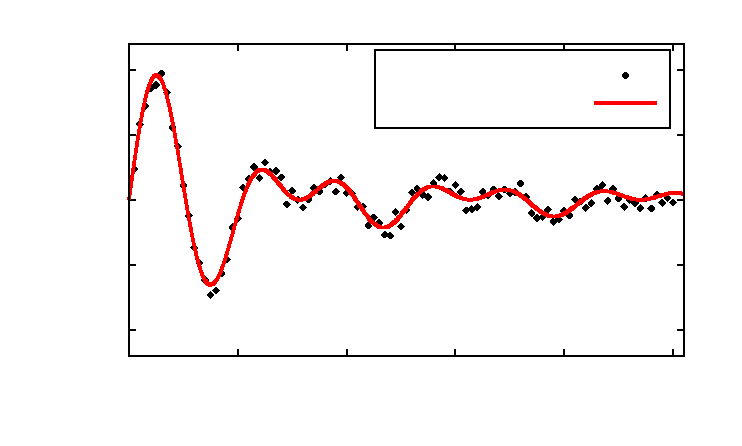
\includegraphics{nonlin-fit-example}}%
    \gplfronttext
  \end{picture}%
\endgroup

				\caption{Beispiel eines nichtlinearen Ausgleichsproblems mit einem freiem Parameter $a$, gegebenen Messwerten und der besten Approximation $f$ mit $a=3.01134$}
				\label{fig:fit-example}
			\end{figure}

		% subsection idee_und_problemstellung (end)

		\subsection{Das Ausgleichsproblem} % (fold)
		\label{sub:das_ausgleichsproblem}
		
			Betrachtet man die obige Problemstellung, ist es hilfreich eine etwas allgemeinere Definition des Ausgleichsproblems zu geben.
			Denn es lassen sich viele Problemstellungen auf ein Solches zurückführen.
			Die Verallgemeinerung soll jedoch darauf beschränkt werden, dass eine beste Approximation gerade im Sinne der Methode der kleinsten Quadrate zu verstehen ist.
			\bigskip

			\begin{definition*}[Ausgleichsproblem, Methode der kleinsten Quadrate]
				Für $n,m\in\SN, m\leq n$, eine gegebene Parametermenge $U\subset\SR^m$ und eine gegebene Residuen-Funktion $r:U\longrightarrow\SR^n$ ist das Ausgleichsproblem definiert durch
				\[ \min \set{\norm{r(\lambda)}^2_2}{\lambda\in U} \]
			\end{definition*}

		% subsection das_ausgleichsproblem (end)

	% section mathematische_grundlagen (end)

	\section{Lösungsverfahren} % (fold)
	\label{sec:l_sungsverfahren}
	
		Im Folgenden seien nun immer $n,m\in\SN, m\leq n$, $U\subset\SR^m$ die gegebene Parametermenge und $r:U\longrightarrow\SR^n$ die Residuen-Funktion, wenn nicht anders behauptet.
		Da wir hier, wie bereits gesagt, nur die Methode der kleinsten Quadrate anwenden, ist es durchaus sinnvoll noch die folgende Funktion zu definieren.
		\[ s:U\longrightarrow[0,\infty),\qquad s := \tfrac{1}{2}\norm{r}_2^2 = \tfrac{1}{2}\transp{r}r \]
		Ist $s$ zweimal stetig differenzierbar, folgt durch Ausrechnen
		\begin{alignat*}{3}
			\nabla s = \transp{\curvb{\Deriv r}}r,\qquad \Deriv\curvb{\nabla s} = \transp{\curvb{\Deriv r}}\Deriv r + \sum_{i=1}^n r_i \Deriv^2r_i
		\end{alignat*}

		\subsection{Gauß-Newton-Verfahren} % (fold)
		\label{sub:gau_newton_verfahren}
		
			Das Gauß-Newton-Verfahren ist ein sogenanntes Quasi-Newton-Verfahren.
			Die grundsätzliche Idee besteht darin, das gegebene Ausgleichsproblem in ein nichtlineares Gleichungssystem umzuformulieren.
			Dieses würde sich dann mit dem bereits bekannten Newton-Verfahren lösen lassen.\\

			Nun zu den Details.
			Wir betrachten ein zwangloses System $U=\SR^m$ von Parametern.
			$r$ sei zweimal stetig differenzierbar.
			Die Lösung des Ausgleichsproblems soll hier gerade durch das Auffinden eines lokalen Minimums $\lambda^\star\in U$ mit den folgenden hinreichenden Bedingungen gegeben sein.
			\begin{tcolorbox}[title=Bedingungen für Minimum, top=0mm]
				\begin{equation}
				\label{eq:gn cond 1}
					\nabla s(\lambda^\star) = 0
				\end{equation}
				\begin{equation}
					\Deriv\curvb{\nabla s}(\lambda^\star) \text{ ist positiv definit}
				\end{equation}
			\end{tcolorbox}
			Durch Einsetzen von $s$ in Bedingung (\ref{eq:gn cond 1}) ergibt sich für das gerade definierte $\lambda^\star\in U$
			\[ \boxb{\transp{\curvb{\Deriv r}}r}\curvb{\lambda^\star} = 0 \]
			Dies ist nun ein nichtlineares Gleichungssystem, welches mithilfe des Newton-Verfahren gelöst werden kann.
			Für den $k$-ten Iterationsschritt mit $k\in\SN$ folgt also
			\[ \lambda^{(k+1)} = \lambda^{(k)} + \xi^{(k)} \]
			\[ \boxb{ \transp{\curvb{\Deriv r}}\Deriv r + \sum_{i=1}^n r_i \Deriv^2r_i }\curvb{\lambda^{(k)}} \xi^{(k)} = -\boxb{ \transp{\curvb{\Deriv r}}r }\curvb{\lambda^{(k)}} \]
			Um sich die aufwendige Berechnung der zweiten Ableitung zu sparen, geht man davon aus, dass $r\curvb{\lambda^\star}\approx 0$.
			Damit kann also die Berechnung von $\xi^{(k)}$ in einer geeigneten Umgebung von $\lambda^\star$ durch folgendes ersetzt werden.
			\[ \boxb{ \transp{\curvb{\Deriv r}}\Deriv r }\curvb{\lambda^{(k)}} \xi^{(k)} = -\boxb{ \transp{\curvb{\Deriv r}}r }\curvb{\lambda^{(k)}} \]

			\begin{tcolorbox}[colframe=black,colbacktitle=white,coltitle=black, attach boxed title to top center={yshift=-2mm},enhanced, titlerule=0.1pt, boxrule=0.5pt, breakable, arc=5pt,title=Algorithmus:\quad Gauß-Newton-Verfahren]
				Eingabe: $r:\SR^m\longrightarrow\SR^n,\quad \lambda^{(0)}\in\SR^m$

				\begin{enumerate}[label=\normalfont (\arabic*)]
					\item Setze $k=0$.
					\item Berechne $r\curvb{\lambda^{(k)}}, \Deriv r\curvb{\lambda^{(k)}}$.
					\label{schritt}
					\item Bestimme den Korrekturvektor $\xi^{(k)}$ gemäß
						\[ \boxb{ \transp{\curvb{\Deriv r}}\Deriv r }\curvb{\lambda^{(k)}} \xi^{(k)} = -\boxb{ \transp{\curvb{\Deriv r}}r }\curvb{\lambda^{(k)}} \]
					\item Setze $\lambda^{(k+1)} = \lambda^{(k)} + \xi^{(k)}$.
					\item Setze $k=k+1$.
					\item Gehe zu Schritt \ref{schritt}, wenn
						\[ k < k_\m{max} \quad \wedge \quad \norm{\xi^{(k)}}_2^2 > \delta_\m{min} \]
				\end{enumerate}
			\end{tcolorbox}

		% subsection gau_newton_verfahren (end)

		\subsection{Levenberg-Marquardt-Verfahren} % (fold)
		\label{sub:levenberg_marquardt_verfahren}
		
			Das Levenberg-Marquardt-Verfahren stellt eine Erweiterung des Gauß-Newton-Verfahrens dar.


			\begin{tcolorbox}[colframe=black,colbacktitle=white,coltitle=black, attach boxed title to top center={yshift=-2mm},enhanced, titlerule=0.1pt, boxrule=0.5pt, breakable, arc=5pt,title=Algorithmus:\quad Levenberg-Marquardt-Verfahren]
				Eingabe: $r:\SR^m\longrightarrow\SR^n,\quad \lambda^{(0)}\in\SR^m$

				\begin{enumerate}[label=\normalfont (\arabic*)]
					\item Setze $k=0$.
					\item Berechne $r\curvb{\lambda^{(k)}}, \Deriv r\curvb{\lambda^{(k)}}$.
					\label{lm-schritt}
					\item 
					\label{lm-corr}
					Bestimme den Korrekturvektor $\xi^{(k)}$ gemäß
						\[ \boxb{ \transp{\curvb{\Deriv r}}\Deriv r + \mu^2\idmat }\curvb{\lambda^{(k)}} \xi^{(k)} = -\boxb{ \transp{\curvb{\Deriv r}}r }\curvb{\lambda^{(k)}} \]
					\item Berechne $\varepsilon_\mu$ und teste, ob die Korrektur akzeptabel ist.
						\[ \varepsilon_\mu = \frac{ \norm{r\curvb{\lambda^{(k)}}}^2_2 - \norm{r\curvb{\lambda^{(k)}+\xi^{(k)}}}^2_2 }{ \norm{r\curvb{\lambda^{(k)}}}^2_2 - \norm{r\curvb{\lambda^{(k)}} + \Deriv r\curvb{\lambda^{(k)}}\xi^{(k)}}^2_2 } \]
						\begin{enumerate}[label=\normalfont (\roman*)]
							\item Fall $\varepsilon_\mu \leq \beta_0$: Setze $\mu = 2\mu$ und gehe zu \ref{lm-corr}.
							\item Fall $\varepsilon_\mu \geq \beta_1$: Setze $\mu = \frac{\mu}{2}$.
						\end{enumerate}
					\item Setze $\lambda^{(k+1)} = \lambda^{(k)} + \xi^{(k)}$.
					\item Setze $k=k+1$.
					\item Gehe zu Schritt \ref{lm-schritt}, wenn
						\[ k < k_\m{max} \quad \wedge \quad \norm{\xi^{(k)}}_2^2 > \delta_\m{min} \]
				\end{enumerate}
			\end{tcolorbox}

		% subsection levenberg_marquardt_verfahren (end)

		\subsection{Simulated Annealing} % (fold)
		\label{sub:simulated_annealing}

			Simulated Annealing stellt ein Verfahren dar, welches im Vergleich zu den zuvor genannten Verfahren ein anderen Ansatz verfolgt.
			Anstatt sich auf das lokale Minimum zu beschränken, versucht es mithilfe von Zufallszahlen das globale Minimum ausfindig zu machen.
			
		
			\begin{tcolorbox}[colframe=black,colbacktitle=white,coltitle=black, attach boxed title to top center={yshift=-2mm},enhanced, titlerule=0.1pt, boxrule=0.5pt, breakable, arc=5pt,title=Algorithmus:\quad Simulated Annealing]
				Eingabe: $r:\SR^m\longrightarrow\SR^n,\quad \lambda_0\in\SR^m$

				\begin{enumerate}[label=\normalfont (\arabic*)]
					\item Berechne $c_0 = \norm{ r\curvb{ \lambda_0 } }_2^2$.
					\item Setze $T = T_0$ und $i=0$.
					\item \label{sa-for} Bestimme einen zufälligen Parameter $\lambda_1$.
					\item Berechne $c_1 = \norm{ r\curvb{ \lambda_1 } }_2^2$.
					\item
						\begin{itemize}
							\item Fall $c_1 < c_2$: Setze $\lambda_0 = \lambda_1$.
							\item Fall $c_1 \geq c_2$: Berechne
								\[ p = \exp\curvb{ \frac{c_0 - c_1}{T} } \]
								und setze $\lambda_0 = \lambda_1$ mit Wahrscheinlichkeit $p$. 
						\end{itemize}
					\item Setze $i=i+1$ und gehe zu Schritt \ref{sa-for}, wenn $i < i_\m{max}$.
					\item Setze $T=\alpha T$ und gehe zu Schritt \ref{sa-for}, wenn $T > T_\m{min}$.
				\end{enumerate}
			\end{tcolorbox}

			\begin{tcolorbox}[colframe=black,colbacktitle=white,coltitle=black, attach boxed title to top center={yshift=-2mm},enhanced, titlerule=0.1pt, boxrule=0.5pt, breakable, arc=5pt,title=C++-Implementierung:\quad Curve Fitting mit Simulated Annealing]
				\lstinputlisting[style = std, language=c++]{../code/src/sa-fit.cpp}
			\end{tcolorbox}

		% subsection simulated_annealing (end)

	% section l_sungsverfahren (end)

	\section{Referenzen} % (fold)
	\label{sec:referenzen}

		\begin{itemize}[label=$\circ$]
			\item Hermann, \textit{Numerische Mathematik}, 3.Auflage
			\item \url{http://en.wikipedia.org/wiki/Gauss-Newton_algorithm}
			\item \url{http://en.wikipedia.org/wiki/Levenberg-Marquardt_algorithm}
			\item \url{http://en.wikipedia.org/wiki/Simulated_annealing}
			\item Funken, \textit{Numerik III}, Skript Universität Ulm, 2012/2013
			\item \url{katrinaeg.com/simulated-annealing.html}
			\item Kincaid und Cheney, \textit{Numerical Analysis}, 3.Edition
		\end{itemize}

	% section referenzen (end)

\end{document}
	